\chapter{Human MS-based Protein expression landscape}
\label{ch:proteomics}

\section{Introduction}


(1) Etat des lieux méthode 1
(2) En travaillant sur l'integration 
3) Etat des lieux méthode 2



Under the impulse of \jyoti, \james\ has reprocessed \enquote{more diverse}
large-scale \ms-based proteomic studies on normal human tissues to this day.

See \Cref{sec:ProteoData} for more details about the details of the datasets and
the pipeline.

See \Cref{subsec:distribPlot} and more particularly \Cref{fig:densityCutler_log2,%
fig:densityKuster_log2,fig:densityPandey_log2}

After exploring the transcriptomic side (way more data) I have explored the
proteomic (\ms-based) before integrating the trancriptomic to the proteomic.
It seems to be the obvious/sensible thing to do.

\begin{figure}[htpb]
    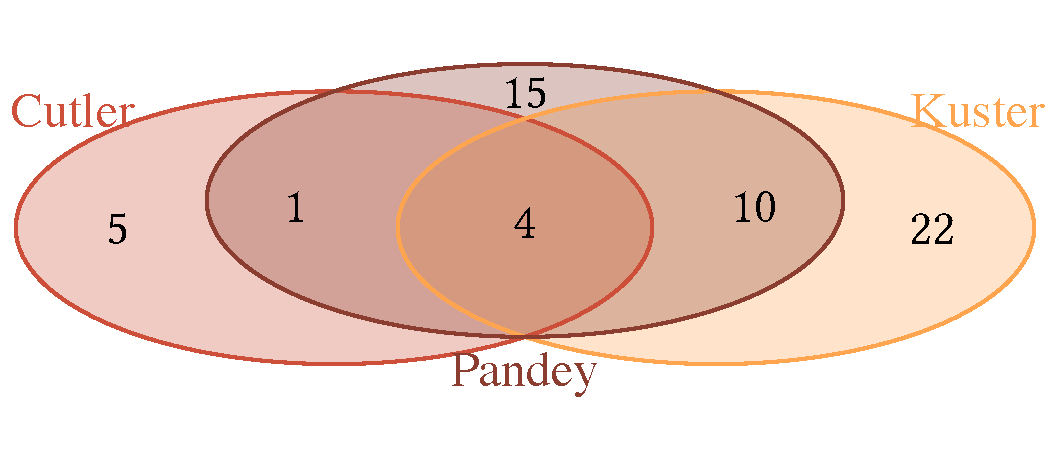
\includegraphics[scale=0.5]{proteomics/VennDiagProtCond.pdf}\centering
    \caption[Distribution of unique shared tissues between
    the 3 MS-based proteomic studies]{\label{VennDiagProt3}\textbf{Distribution
    of unique and shared tissues between the 3 \ms{}-based proteomic studies.}}
\end{figure}

\section{Results}

\subsection{Limited availability (and overlap) of tissues}




\subsection{Disparate universe: High-throughput proteomics has a greater
variability of detection and quantification than high-throughput transcriptomics}

It is more about identification than quantification.

\subsection{About half of the quantified proteins for a given tissue are found
in different datasets}

\subsection{Technical variability seems to prevail over biological signal:
correlations between samples from a same tissue are globally lesser than
correlation between samples from a same study.}


\section{Discussion}


%%%% Maybe?
%%%Quantification with the first method
%%%Quantification with the second method with PPKM
%%%%



\section{White Board}

Less things to do than for transcriptomics.

\minisec{intro}
While \ms\ older techniques there are not tissues datasets before a couple of
years ago (2014 for Pandey, Kuster) while 2010 for Cutler.


Put the two Venn Diagrams (tissues, proteins expressed).

Cutler: older and no publication,
hard to know exactly what were the methodological protocols;but then we need to
be sure.

Super set of proteins: they are expressed in every tissues.

And then the tissues spe proteins: the one that are found in the same tissues
over the three datasets.


Less things to do than transcriptomics

Conclusion Proteomics: Very hard to quantify;

Need to use Pandey (as it is the best for the analysis:
greater range of expressed proteins); pooled people (3, 2 males and one female)
and confere chapter expressed: they have better expression profile shapes.




